\section{Discretization of the FDS pressure equation}
\label{SEC_discretization}
The pressure equation in FDS, an elliptic partial differential equation of second order which is commonly referred to as {\it Poisson equation}, reads as
\be 
  \nabla^2 \cH =-\dod{(\nabla \cdot {\bf u})}{t} - \nabla \cdot \bF\,.
  \label{EQ_pressure}
\ee
%
Detailed information on its derivation can be found in in the FDS Technical Reference Guide \cite{McGrattan:2018:TG}.
The pressure term $\cH \equiv |\bu|^2/2 + \tp/\rho$  incorporates the density $\rho$ as well as the perturbation pressure $\tp$ by which the fluid motion is driven. Obviously, $\cH$ is strongly coupled with the velocity field
$\bu$ and the force term $\bF$ which includes the thermodynamic contributions from the previous time step such as radiation, combustion, pyrolysis, etc. Thus, 
the quality of the pressure solution is of great importance for the accuracy of the entire numerical scheme in FDS.

In order to obtain a corresponding system of equations which can be solved on a computer system the
spatial derivative of $\hp$  in Equation (\ref{EQ_pressure})  is discretized by a cell-centered {\it finite difference method} of second-order accuracy. Its numerical solution requires the specification of appropriate boundary conditions and has to be done at least twice in every step of the FDS time marching scheme, namely in the respective predictor and corrector parts.
%
The efficient parallelization of Equation (\ref{EQ_pressure}) must necessarily ensure that the strong global coupling induced by the underlying elliptic character is mapped as closely as possible.

\subsection{Global versus local discretization}

\label{SEC_poisson}

In order to describe the basic functionality of the various Poisson solvers in FDS,
Figure \ref{FIG_basic_pipe_geometry} introduces a simple pipe-shaped geometry in 2D with a small internal obstruction, a prescribed inflow from the left, an open outflow on the right and a middle pressure device. This so-called {\ct poisson2d} geometry will be used as a  demonstration case throughout the entire paper. 

\begin{figure}[h]
\begin{center}
\input{\tikzPath/single_pipe_nogrid_obst.tex}
\end{center}
\caption[Simple pipe-shaped geometry in 2D]{Simple pipe-shaped 2D-geometry {\ct poisson2d} with an internal obstruction, a prescribed inflow from the left, a measuring point for the pressure and an open outflow on the right.}
\label{FIG_basic_pipe_geometry}
\end{figure}

\newpage
If the whole domain is discretized in one piece, one global system of equations is 
obtained,
\be 
  Ax = b\,, 
  \label{EQ_SCARC_single_system}
\ee
where $n$ is the number of total grid cells, 
$x, \,b\in\mathbb{R}^n$ denote the corresponding solution and right hand side vectors and $A \in \mathbb{R}^{n \times n}$ the overall Poisson matrix. 

However, since FDS is limited to cubic or rectangular meshes, typically a subdivision into $M$ individual sub-meshes is used with $n_m$ local cells each. In this case every sub-mesh holds its own system of equations 
\be 
   A_i x_i = b_i\,, \qquad i=1, \ldots, M, 
  \label{EQ_SCARC_multi_system}
\ee
with corresponding local solution and right hand side vectors $x_i, b_i \in \mathbb{R}^{n_i}$ and locally defined Poisson matrices $A_i \in \mathbb{R}^{n_i\times n_i}$. The resulting global and local discretizations are shown in Figure \ref{FIG_global_vs_local_discretization}.


\begin{figure}[h]
\begin{center}
\input{\tikzPath/single_pipe_grid_obst_Ax=b.tex}\quad\quad
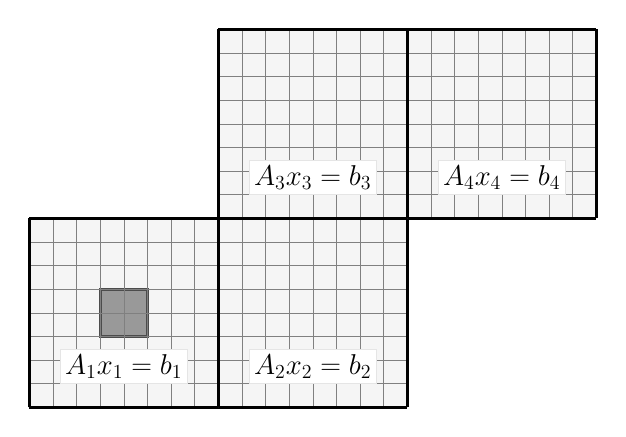
\begin{tikzpicture}
[
scale=0.6,
every node/.style ={scale=0.6},
Background/.style={rectangle,draw=black!04,fill=black!04, thin, minimum size = 4 cm},
Obstruction/.style={rectangle,draw=black!70,fill=black!40, very thick, minimum size=1cm},
Finegrid/.style={step=0.5cm,gray,very thin},
Thickline/.style={-,draw=black!100,fill=black!02, very thick},
Thinline/.style={draw=black!100,fill=black!02, very thin},
Ball/.style={circle, draw=black!40, fill=red!20, thin, minimum size=3.5mm},
Circle/.style={circle,draw=black!40,fill=black!06,thin,minimum size=35.5mm},
%Rectangle/.style={rectangle,color=blue, inner xsep=7pt, inner ysep=7pt,},
%Rectangle/.style={rectangle,color={rgb,255:red,192;green,58;blue,10}, inner xsep=7pt, inner ysep=7pt,},
Rectangle/.style={rectangle,draw=black!10,fill=white,inner xsep=3pt, inner ysep=3pt,},
box/.style = {very thin, rectangle, inner xsep=10pt, inner ysep=10pt,},
]

\node[Background] at (2,2) {};
\node[Background] at (6,2) {};
\node[Background] at (6,6) {};
\node[Background] at (10,6) {};

\node[Obstruction] at (2,2) {};

\draw[Finegrid] (0,0) grid (8,4);
\draw[Finegrid] (4,4) grid (12,8);

\draw[Thickline] (0,0)--(8,0);
\draw[Thickline] (4,8)--(12,8);
\draw[Thickline] (0,4)--(4,4);
\draw[Thickline] (8,4)--(12,4);

\draw[Thickline] (0,0)--(0,4);
\draw[Thickline] (4,8)--(12,8);
\draw[Thickline] (4,4)--(4,8);
\draw[Thickline] (8,0)--(8,4);
\draw[Thickline] (12,4)--(12,8);

\draw[Thickline] (4,0)--(4,4);
\draw[Thickline] (4,4)--(8,4);
\draw[Thickline] (8,4)--(8,8);

\node[Rectangle] at ( 2,0.86) {\LARGE $\boldsymbol{A_1x_1=b_1}$};
\node[Rectangle] at ( 6,0.86) {\LARGE $\boldsymbol{A_2x_2=b_2}$};
\node[Rectangle] at ( 6,4.86) {\LARGE $\boldsymbol{A_3x_3=b_3}$};
\node[Rectangle] at (10,4.86) {\LARGE $\boldsymbol{A_4x_4=b_4}$ };

\vspace{4cm}

%\node[Rectangle] at (16,2) {\textcolor{hhpred} {\Huge $ x \,\overset{ \mbox{\raisebox{1mm}{?}}}{=}\, \summv x_i$}};

\end{tikzpicture}

\end{center}
\caption[Global discretization versus collection of local discretizations]{Different discretization types for the Poisson problem: (Left) Global discretization with one globally defined system of equations $Ax=b$. (Right) Local discretizations with a set of locally defined systems of equations $A_ix_i=b_i$.}
\label{FIG_global_vs_local_discretization}
\end{figure}
Note that a global discretization can also be handled in a multi-mesh context, i.e.\ in a {\it data-parallel} sense. 
For this purpose, each mesh stores the corresponding part of the global matrix as well as the solution and right-side vector. 
By means of suitable data exchanges between adjacent meshes the individual matrix-vector operations are then performed 
in exactly the same way as would also be the case with an actual global execution.

With regard to parallelization the use of local discretizations seems to be the more natural approach. 
Thus, the crucial question is, if there are appropriate solutions strategies for a local discretization 
such that the obtained collection of mesh-wise solutions is comparably good as the overall solution for the corresponding global discretization, i.e. $\sum_{i=1}^M x_i \sim x$\,?
This question will be addressed subsequently based on the example of the Poisson solvers used in FDS.

\subsection{Structured versus unstructured discretization}
Regarding the discretization of internal obstructions two possible approaches must be distinguished as well, which essentially differ in how they treat cells internal to solid objects and their neighboring gas-phase cells. Those different types have their pros and cons and also require different solution strategies which will be explained below.
\newpage
\begin{itemize}
\item A {\bf structured discretization}
explicitly includes both gas-phase and solid cells and is the default type in FDS. The same matrix stencil is applied all over the domain. Without any exception all grid cells are incorporated into the resulting discretization matrix which therefore takes a very regular shape. As a major advantage this strategy allows the use of highly tuned solvers developed specifically for regular grid structures which can be performed with enormous computational efficiency. However, it is not possible to prescribe the required homogeneous no-flux condition at internal boundaries directly. Erroneously, the velocity field may contain non-zero contributions towards internal solids associated with a corresponding loss of accuracy which represents the greatest disadvantage of this strategy.
\item An {\bf unstructured discretization}
only incorporates the gas-phase cells while omitting all solid cells from the system of equations. On gas-phase cells directly adjacent to the surface of an obstruction the homogeneous no-flux Neumann condition can explicitly be specified and included into the matrix so that there are no more penetration errors along internal obstructions. Thus, the major advantage of this strategy is that it offers more flexibility and achieves a higher degree of accuracy. But, in contrast to the structured case it requires the use of individual matrix stencils for the different grid cells depending on their location with respect to obstructions such that the regular matrix shape gets lost. The solution of such an irregular system places significantly higher demands on the robustness of the solver, which can comprehensively limit the achievable efficiency and represents the greatest disadvantage of this methodology.
\end{itemize}
In FDS, both the structured and unstructured discretization type can be used in combination with suitable solution strategies each, as will be shown subsequently.
The differences between both are illustrated in Figure \ref{FIG_structured_vs_unstructured_discretization} 
where the respective matrix stencils are displayed. Both plots therein are related to
the lower left mesh in case of the local discretization containing the internal obstruction as can be seen in the right plot of \ref{FIG_global_vs_local_discretization}.
\begin{figure}[ht]
\begin{center}
\begin{minipage}[b]{0.475\textwidth}
\centering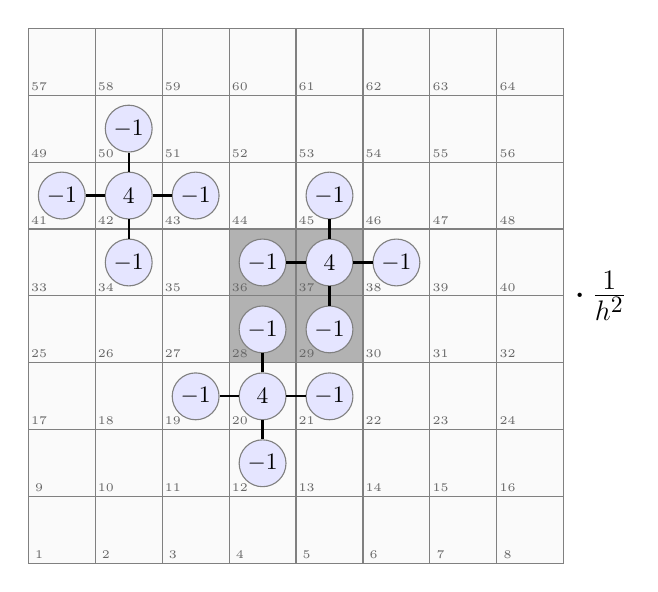
\begin{tikzpicture}
[
 scale=0.85,
 every node/.style ={scale=0.85},
 inner sep=0.5mm,
 BLUECIRC/.style={circle, draw=black!50, fill=blue!10, thin, minimum size=7.0mm},
 REDCIRC/.style={circle, draw=black!50, fill=red!10, thin, minimum size=7.0mm},
 OBST/.style={rectangle, draw=black!50, fill=black!30, thin, minimum size=10mm},
 CELL/.style={rectangle, draw=black!50, fill=black!02,   thin, minimum size=10mm},
 ],
%
\foreach \y in {1,2,3,4,5,6,7,8}
   \foreach \x in {1,2,3,4,5,6,7,8}
      {
        \node [CELL]    at ( \x, \y)  {};
       }
\foreach \y in {4,5}
   \foreach \x in {4,5} { \node [OBST]    at ( \x, \y)  {}; }
%
\node  at (9.0,4.5)  {\LARGE \,$\cdot \,\frac{1}{h^2}$};       
%
\node [BLUECIRC]  (XS)   at ( 4, 2)  {$-1$};
\node [BLUECIRC]  (XW)   at ( 3, 3)  {$-1$};
\node [BLUECIRC]  (XC)   at ( 4, 3)  {$4$};
\node [BLUECIRC]  (XN)   at ( 4, 4)  {$-1$};
\node [BLUECIRC]  (XE)   at ( 5, 3)  {$-1$};
%
\node [BLUECIRC]  (YS)   at ( 2, 5)  {$-1$};
\node [BLUECIRC]  (YW)   at ( 1, 6)  {$-1$};
\node [BLUECIRC]  (YC)   at ( 2, 6)  {$4$};
\node [BLUECIRC]  (YN)   at ( 2, 7)  {$-1$};
\node [BLUECIRC]  (YE)   at ( 3, 6)  {$-1$};
%
\node [BLUECIRC]  (ZS)   at ( 5, 4)  {$-1$};
\node [BLUECIRC]  (ZW)   at ( 4, 5)  {$-1$};
\node [BLUECIRC]  (ZC)   at ( 5, 5)  {$4$};
\node [BLUECIRC]  (ZN)   at ( 5, 6)  {$-1$};
\node [BLUECIRC]  (ZE)   at ( 6, 5)  {$-1$};
%
\draw [thick]  (XC.south)  -- (XS.north) ;
\draw [thick]  (XC.west)   -- (XW.east) ;
\draw [thick]  (XC.north)  -- (XN.south) ;
\draw [thick]  (XC.east)  -- (XE.west) ;
%
\draw [thick]  (YC.south)  -- (YS.north) ;
\draw [thick]  (YC.west)   -- (YW.east) ;
\draw [thick]  (YC.north)  -- (YN.south) ;
\draw [thick]  (YC.east)  -- (YE.west) ;
%
\draw [thick]  (ZC.south)  -- (ZS.north) ;
\draw [thick]  (ZC.west)   -- (ZW.east) ;
\draw [thick]  (ZC.north)  -- (ZN.south) ;
\draw [thick]  (ZC.east)  -- (ZE.west) ;
%
\foreach \y in {0,1,2,3,4,5,6,7} {
  \pgfmathsetmacro{\ypos}{(\y+0.63)}
  \foreach \x in {0,1,2,3,4,5,6,7} {
    \pgfmathsetmacro{\xpos}{(\x+0.66)}
    \pgfmathsetmacro{\num}{int(8*\y+\x+1)}
    \draw[color=black!60]   node at (\xpos,\ypos) {\tiny \num};
  }
}
%
\end{tikzpicture}


\end{minipage}
\hspace{5mm}
\begin{minipage}[b]{0.475\textwidth}
\centering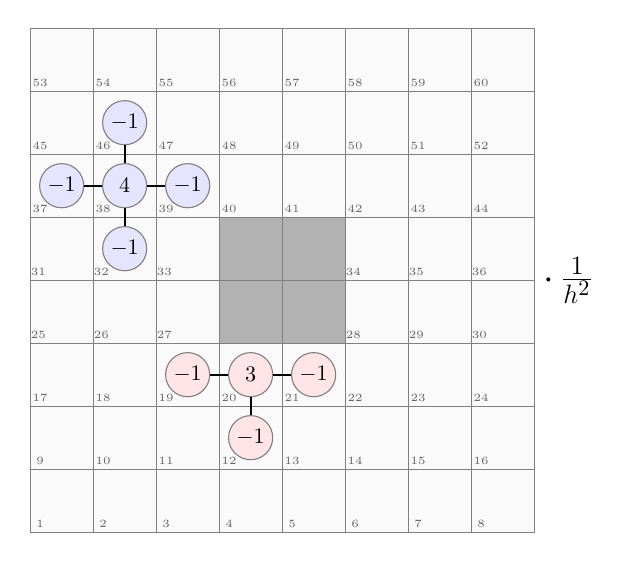
\begin{tikzpicture}
[
 scale=0.8,
 every node/.style ={scale=0.8},
 inner sep=0.5mm,
 BLUECIRC/.style={circle, draw=black!50, fill=blue!10,  thin, minimum size=7.0mm},
 REDCIRC/.style={circle, draw=black!50, fill=red!10, thin, minimum size=7.0mm},
 OBST/.style={rectangle, draw=black!50, fill=black!30, thin, minimum size=10mm},
 CELL/.style={rectangle, draw=black!50, fill=black!02,   thin, minimum size=10mm},
 ],
%      
\foreach \y in {1,2,3,4,5,6,7,8}
   \foreach \x in {1,2,3,4,5,6,7,8}
      {
        \node [CELL]    at ( \x, \y)  {};
       }
\foreach \y in {4,5}
   \foreach \x in {4,5} { \node [OBST]    at ( \x, \y)  {}; }
%
\node  at (9.0,4.5)  {\LARGE \,$\cdot \,\frac{1}{h^2}$};       
%
\node [REDCIRC]  (XS)   at ( 4, 2)  {$-1$};
\node [REDCIRC]  (XW)   at ( 3, 3)  {$-1$};
\node [REDCIRC]  (XC)   at ( 4, 3)  {$3$};
\node [REDCIRC]  (XE)   at ( 5, 3)  {$-1$};
%
\node [BLUECIRC]  (YS)   at ( 2, 5)  {$-1$};
\node [BLUECIRC]  (YW)   at ( 1, 6)  {$-1$};
\node [BLUECIRC]  (YC)   at ( 2, 6)  {$4$};
\node [BLUECIRC]  (YN)   at ( 2, 7)  {$-1$};
\node [BLUECIRC]  (YE)   at ( 3, 6)  {$-1$};
%
\draw [thick]  (XC.south) -- (XS.north) ;
\draw [thick]  (XC.west)  -- (XW.east) ;
\draw [thick]  (XC.east)  -- (XE.west) ;
%
\draw [thick]  (YC.south) -- (YS.north) ;
\draw [thick]  (YC.west)  -- (YW.east) ;
\draw [thick]  (YC.east)  -- (YE.west) ;
\draw [thick]  (YC.north) -- (YN.south) ;
%
\pgfmathsetmacro{\num}{int(0)}
\foreach \y in {0,1,2} {
  \pgfmathsetmacro{\ypos}{(\y+0.63)}
  \foreach \x in {0,1,2,3,4,5,6,7} {
    \pgfmathsetmacro{\xpos}{(\x+0.66)}
    \pgfmathsetmacro{\num}{int(8*\y+\x+1)}
    \draw[color=black!60]   node at (\xpos,\ypos) {\tiny \num};
  }
}
%
\draw[color=black!60]   node at (0.63,3.63) {\tiny 25};
\draw[color=black!60]   node at (1.63,3.63) {\tiny 26};
\draw[color=black!60]   node at (2.63,3.63) {\tiny 27};
\draw[color=black!60]   node at (5.63,3.63) {\tiny 28};
\draw[color=black!60]   node at (6.63,3.63) {\tiny 29};
\draw[color=black!60]   node at (7.63,3.63) {\tiny 30};
%
\draw[color=black!60]   node at (0.63,4.63) {\tiny 31};
\draw[color=black!60]   node at (1.63,4.63) {\tiny 32};
\draw[color=black!60]   node at (2.63,4.63) {\tiny 33};
\draw[color=black!60]   node at (5.63,4.63) {\tiny 34};
\draw[color=black!60]   node at (6.63,4.63) {\tiny 35};
\draw[color=black!60]   node at (7.63,4.63) {\tiny 36};
%
\foreach \y in {5,6,7} {
  \pgfmathsetmacro{\ypos}{(\y+0.63)}
  \foreach \x in {0,1,2,3,4,5,6,7} {
    \pgfmathsetmacro{\xpos}{(\x+0.66)}
    \pgfmathsetmacro{\num}{int(8*\y+\x-3)}
    \draw[color=black!60]   node at (\xpos,\ypos) {\tiny \num};
  }
}
%
\end{tikzpicture}

\end{minipage}
\end{center}
\caption[Structured versus unstructured discretization]{Matrix stencils for both discretization types: (Left) The structured discretization uses the same matrix stencil everywhere, including cells internal to the obstruction. (Right) The unstructured discretization uses individual matrix stencils, excluding all cells internal to the obstruction.}
\label{FIG_structured_vs_unstructured_discretization}
\end{figure}

Figure \ref{FIG_structured_vs_unstructured_spy} opposes the sparsity patterns of the resulting Poisson matrices to each other.
As can be seen clearly, both discretization types lead to sparse matrices which basically have only very less non-zero elements. Based on the underlying stencils the non-zeros are restricted to only a few diagonal bands (5 in 2D, 7 in 3D)
which is very less compared to the number of possible entries.
\begin{figure}[h]
\begin{center}
\includegraphics[width=0.35\textwidth]{\figPath/structured_spy.png}\hspace{1.6cm}
\includegraphics[width=0.35\textwidth]{\figPath/unstructured_spy_zoom.png}
\end{center}
\caption[Structured versus unstructured sparsity pattern]{Sparsity patterns for the resulting Poisson matrices: (Left) The structured discretization leads to a completely regular pattern. (Right) The unstructured discretization shows irregularities related to the internal obstruction .}
\label{FIG_structured_vs_unstructured_spy}
\end{figure}

However, the structured discretization results in a highly regular matrix with a constantly repeating pattern while the unstructured discretization shows irregularities associated with the different treatment of the internal obstruction as indicated with the red circle in the right plot of Figure \ref{FIG_structured_vs_unstructured_spy}. 
For a simple obstruction like the one considered here, the differences are not big, but the situation is completely different for more realistic applications with complex geometric details. In any case, the mentioned optimized solvers for regular grids can no longer be applied in the unstructured case.
Note, that the unstructured discretization even leads to a smaller dimensioned matrix since the obstruction is not included in the discretization process. But this supposed advantage typically does not carry weight due to the more complex structure as a whole.

